%#BIBTEX pbibtex aiit_bulletin
%% 産業技術大学院大学紀要フォーマット
%% Created: 2013-06-30 Y.Chubachi
\documentclass[a4j, 12Q, twocolumn, twoside]{jsarticle}
\usepackage{aiit_bulletin}		% 紀要のスタイル

%%
%% 1.必要に応じてパッケージやマクロをここに追加
%%
\usepackage{newcent}			% Centuryフォント
\usepackage[dvipdfmx]{graphicx}		% 図の取り込み(PDF対応)用
\usepackage{okumacro}			% ルビ・圏点など
\usepackage{url}			% URLの出力

%%
%% 2.英語論文の場合は下記2行のコメントを外してください
%%

% \renewcommand{\tablename}{Table~}
% \renewcommand{\figurename}{Fig.~}

%%
%% 3.タイトルを設定してください
%%
%% 本文が英文の場合は,\etitle, \eauthorを削除し,\titleと\autherに
%% 英文を記入してください.
%%

%%
%% 和文表題
%% 
\title{enPiTプログラムにおける遠隔PBLとアジャイル教材開発}

%%
%% 和文著者名
%%
%% \thanksの中で改行する場合\\ではなく\newlineを使用する
%%
\author{
  中鉢 欣秀
  \thanks{産業技術大学院大学 \newline
  Advanced Institute of Industrial Technology}
}

%%
%% 英文表題
%%
\etitle{Project-based Distance Learning in enPiT Program \\
  and Agile Teaching Material Development}

%%
%% 英文著者名
%%
\eauthor{
  Yoshihide Chubachi
  \thanksmark[1]
}

%%
%% 英文アブストラクト
%%
\begin{abstract}
Project-based distance learning is to develop software engineers who can work with project members at distant places.  We have provided such educational environment in AIIT PBL.  In this paper, we will discuss two points of views as following.  1) Cloud base software development tools for this kind of learning.  2) Agile teaching material development with novel video studio.  The combination of these concepts improves the efficiency of PBL for the students who want to learn pragmatical software engineer skills.
\end{abstract}

%%
%% 英文キーワード
%%
\keywords{Project-based distance learning, PBL, Agile studio}

%%
%% 受領日
%%
\receivedon{2014-10-03}

% \renewcommand{\topfraction}{1.0}
% \renewcommand{\bottomfraction}{1.0}
\renewcommand{\dbltopfraction}{1.0}
% \renewcommand{\textfraction}{0.01}
% \renewcommand{\floatpagefraction}{1.0}
\renewcommand{\dblfloatpagefraction}{1.0}
\setcounter{topnumber}{5}
\setcounter{bottomnumber}{5}
\setcounter{totalnumber}{10}

\renewcommand{\topfraction}{.85}
\renewcommand{\bottomfraction}{.60}
\renewcommand{\textfraction}{.15}
\renewcommand{\floatpagefraction}{.6}

\begin{document}
%%
%% 4.タイトルを出力
%%
%% \maketiteleにあるオプション[0pt]はタイトルと本文の間隔
%% を調整するものです.
%% 1ページ目の脚注の下端と本文の下端が左右の段で揃わない
%% とき,この値を0pt〜8ptくらいの範囲で調整してください.
\amaketitle[-1pt]

%%
%% 5.本文
%%
\section{はじめに}

産業技術大学院大学(以下,AIIT)では,従来よりベ
トナム国家大学UETとの遠隔PBLを実施してき
た\cite{酒瀬川泰孝:2013, 木崎悟2012国際, 木崎:2011:チ
  ケット駆動, 木崎悟:2011-05-10, Nishino:2010,
  pub:tozawa-global-2009, 大類優子:2009}.2013年
度から始まったenPiTプログラム\cite{wired:2014,
  enPiT_aiit:2013, enPiT:2012:about}では,琉球大
学の学生との協働PBLや社会人が自宅からPBLに参加す
ることを想定した遠隔PBLが行われている.

本論文では,ソフトウエア開発を行うPBLを遠隔からも
円滑に参加できるようにするための,各種のクラウド
型のツールについて考察する.また,PBLに参加してい
る学習者が事前学習のための教材として利用する動画
教材を迅速に開発することを木テクとして現在構築中
の「アジャイル教材開発スタジオ」について紹介す
る.

なお,本論文は2014 PCカンファレンスの発表論文をも
とに発展させたものである.

\section{enPiTにおける遠隔PBL}
\subsection{プログラムの全体像}
従来のソフトウエア開発型PBL(Project Besed
Learning)は教室等で実施し,face to faceによるグ
ループワークの形態で行うことが多かった.しかしな
がら,実務におけるソフトウエア開発では,遠隔地に
いるプロジェクトメンバーと協働で開発プロセスを遂
行する例も多く見られる.特に,近年ではオフショア
開発ということで,海外のメンバーと英語等でコミュ
ニケーションしながらソフトウエアを共同開発する場
合も多い.

AIITでは,このようなソフト
ウエア開発体制の多様化を踏まえ,海外の大学(ベト
ナム国家大学)や,国内遠隔地(琉球大学)の学生と
共に,分散型でのソフトウエア開発を経験できるPBLを
行っている.

遠隔地との分散PBLを実施すると,開発プ
ロセスやコミュニケーションにおいて発生する課題が,
従来のPBLよりも更に強調されることになる.このこと
は,学生に対してPBLで解決すべき課題の難易度を高め
ることにつながり,開発の経験者にとっても挑戦しが
いのある,実りの多いPBLとなる.

本発表では,これまでに遠隔地とのPBLを実施して得た
知見のうち,クラウド型のソフトウエア開発環境の活
用について焦点を当てて論じたい.これらのツールを
活用して実施している本学での分散PBLについて述べ,
今後の地方教育への展開についても考察する.

\subsection{遠隔PBLのための事前学習}

遠隔地とのソフトウエア開発プロジェクトを,PBL教育
の一環として実施するには,参加する学生に,共同開
発のために利用する開発ツールについての事前学習を
しておくことを推奨する.

PBLのために何らかの事前学習を行うということには,
議論がある.ある知識を学習する必要性は,学習者が
プロジェクト実施中に対面する実課題を経験すること
で認識する.従って,プロジェクトの実施中に,学習
者が知識取得の必要性を認識した後,勉強をすること
が効果的である,という考え方もある.

しかしながら,遠隔地とのソフトウエア開発において
は,これらのツールの使用方法について事前に学んで
置かないと,そもそもの開発プロジェクトのスタート
ラインに立てない.

また,優れたツールには先人が問題解決のために実装
した多くの知恵が詰まっている.教員は予め学習者に
ツールについて事前学習を行い,一定の理解をさせて
おく.そして,プロジェクトで実際に使用することで
より,ツールの機能についてその本質的意義を更に深
く認識できるとう効果が期待できる.

\subsection{遠隔地とのPBLで利用するツール}
本研究では,ソフトウエア開発環境として,言語処理
系やOSの基本操作は既に知っているものと仮定する.
その上で,特に遠隔地とのプロジェクトのために押さ
えておきたい,分散開発環境について事前に学習すべ
き事柄について論じる.

分散型の開発では,複数のソースコードファイルから
構成されるソフトウエアを,様々な場所にいる開発者
が同時並行で実装していくことになる.これを実現す
るためには,分散型のバージョン管理システムを利用
することが一般的だ.

近年,ソフトウエア開発者が特に注目しているのが
「Git」と呼ばれるバージョン管理システムであり,そ
のリポジトリを一定の制限のもと無料で利用できる
「GitHub」と呼ばれるクラウド型のシステムである.

分散型のバージョン管理システムには,他にも古くか
ら利用されているCVS(Concurrent Versions System)
やSVN(Subversion)は有名だ.PBLにおいてこれらを
利用しているケースも多い.

\begin{figure*}
 \centering
 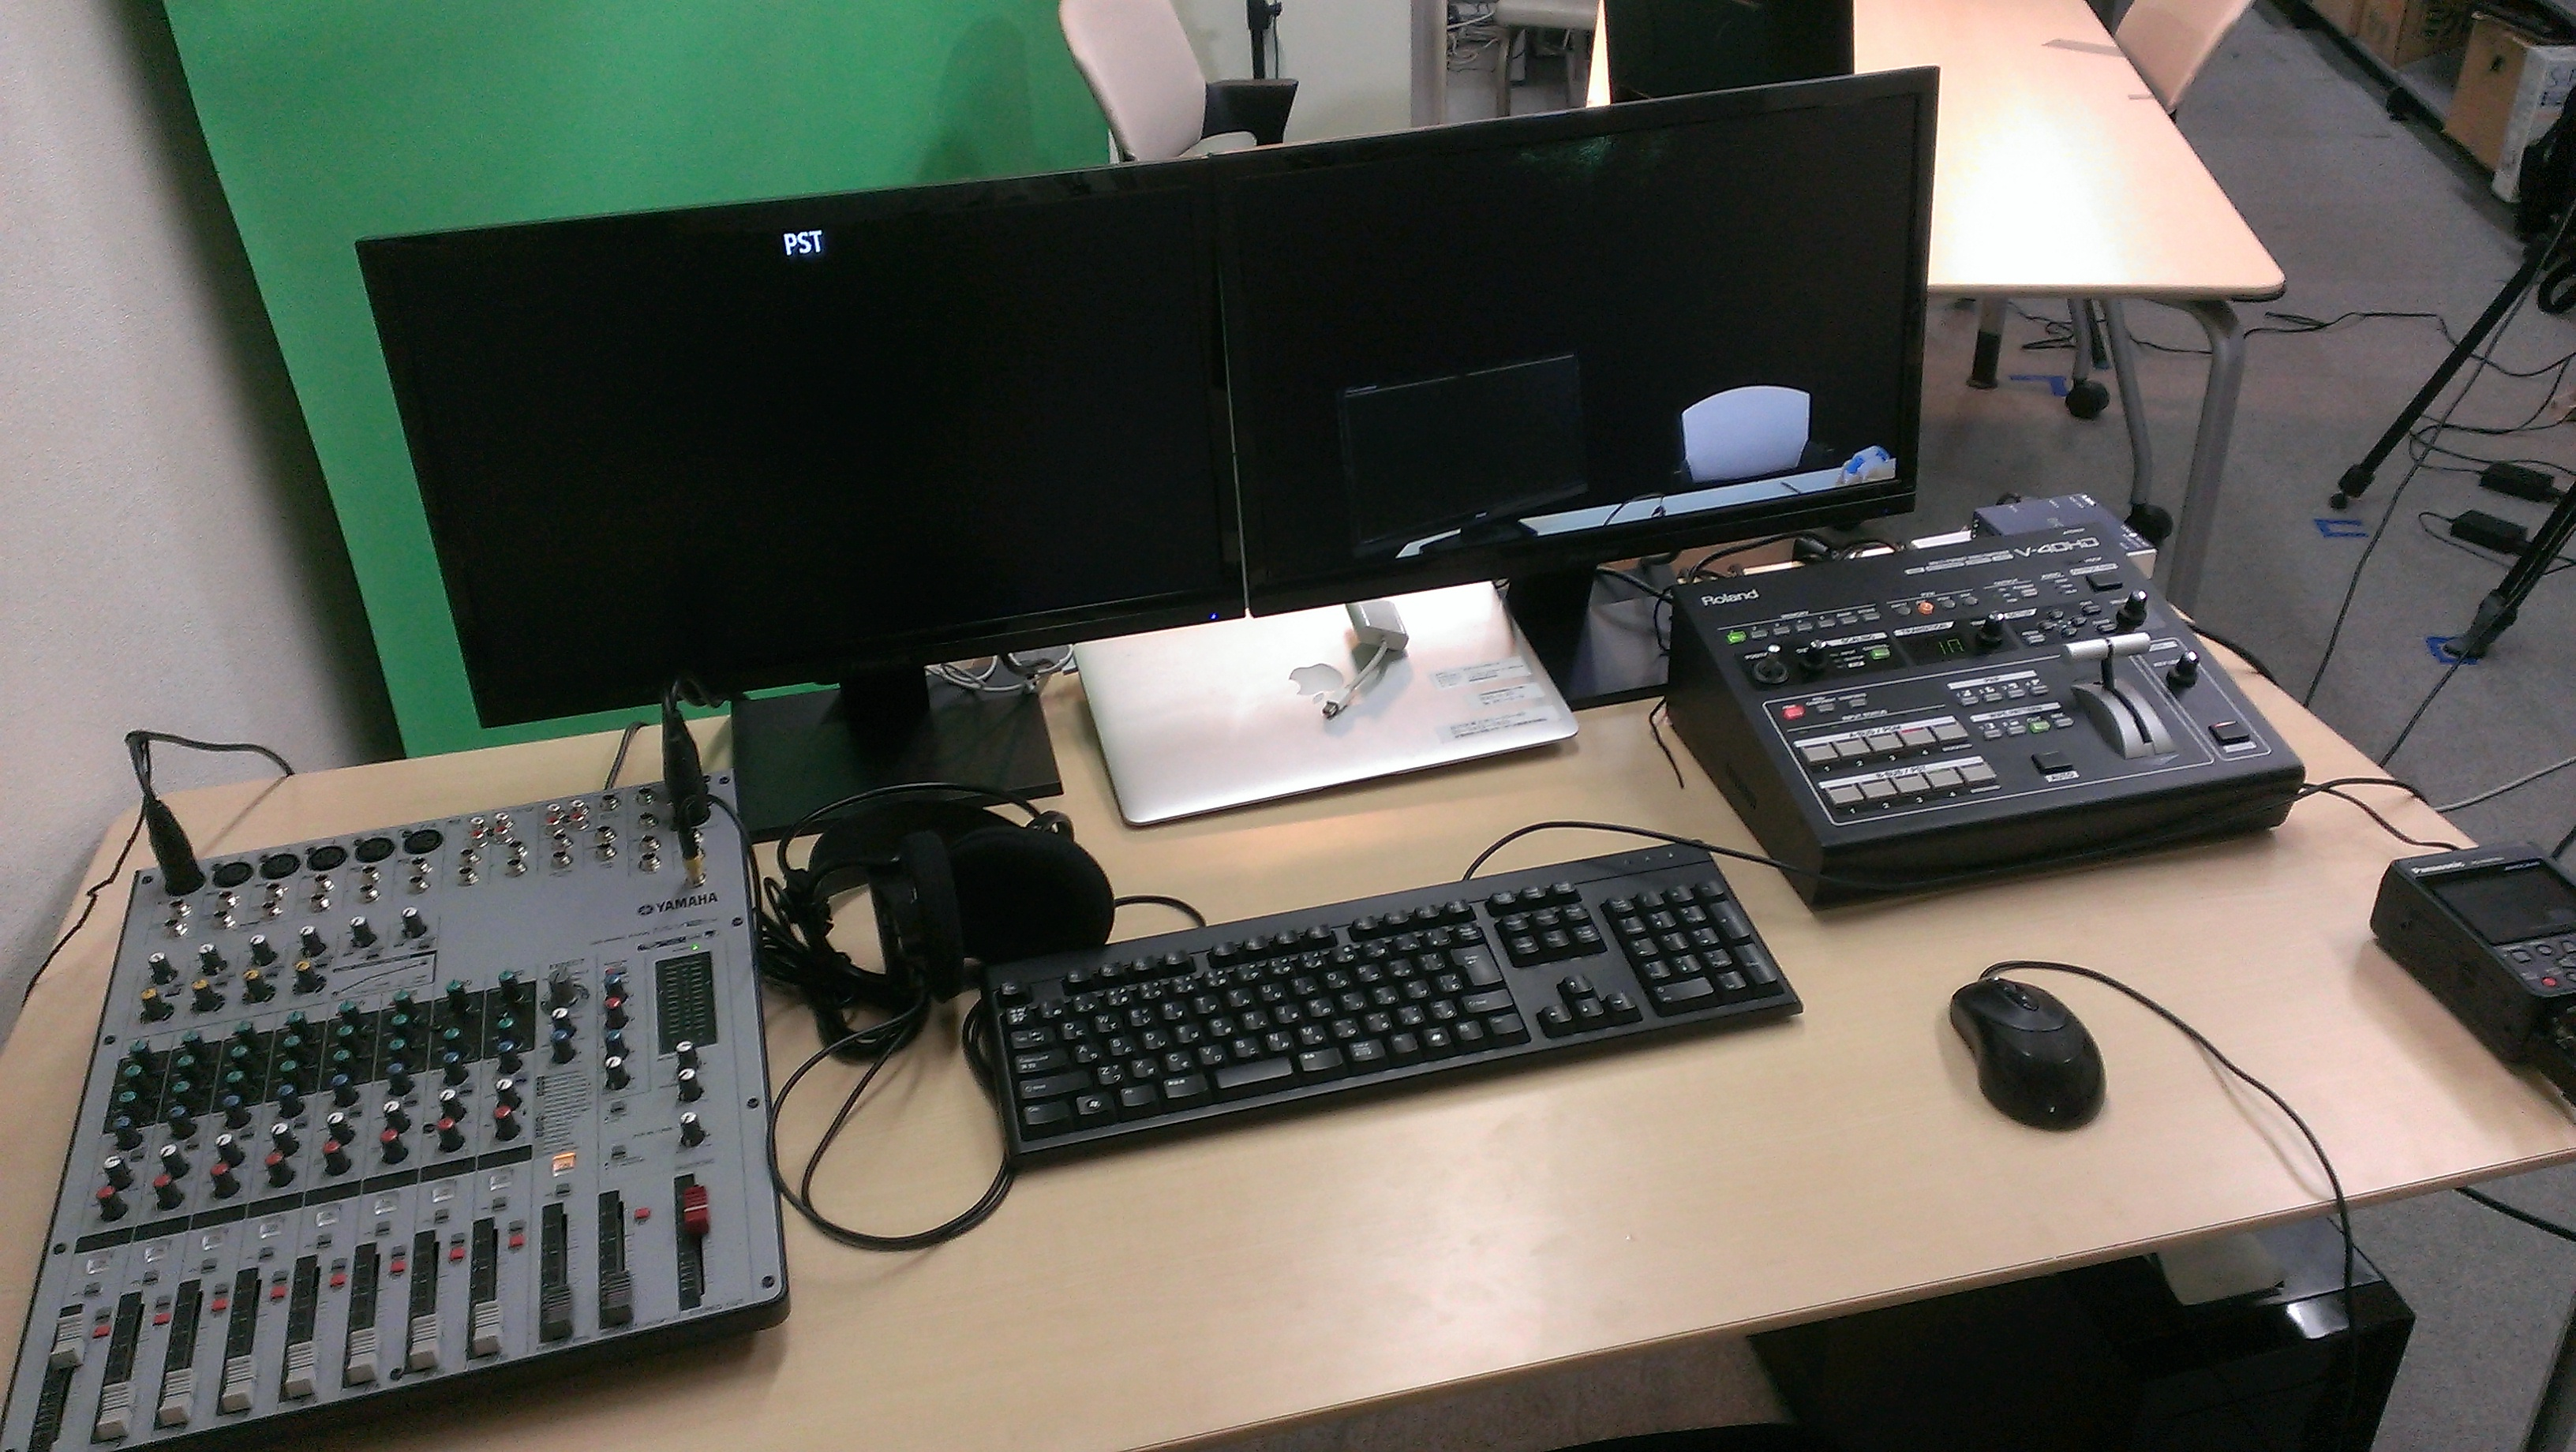
\includegraphics[width=\linewidth]{figures/switcher.jpg}
 \caption{映像スイッチャー及び音声ミキサー}
 \label{fig:switcher}
\end{figure*}

\subsection{Gitの特徴}
ここで,他のシステムではな
く,Git及びGitHubをPBLのために事前学習させること
の狙いについて述べる.Gitは,Linuxの開発者であ
るLinus Torvaldsが開発した.

Linuxと言えば,オープンソース型のソフトウエア開発
として最も巨大なものの一つである.このプロジェク
トのバージョン管理のために,比較的最近であ
る2005年になってLinus自らGitというツールを改めて
開発したことは興味深い.

他の類似するシステムが既に存在するにも関わら
ず,Linusが新たなツールを開発しなくてはならなかっ
たのは,既存の他のツールでは満足できなかったから
だという.

そこに新たに開発されたGitには,大量のソースコード
のバージョンを長年管理し,世界的なオーブンソース
開発を行ってきたLinus及び開発コミュニティの豊富な
知見が含まれていると見るべきである.

実際に,Gitに触れてみると,このことがよく分かる.
一例として,Gitにおいて,ソースコードを変更したと
きの差分を管理するための「コミット」という概念に
ついて述べる.

Gitでは,この「コミット」に基づき,ブランチやマー
ジと行った各種の機能を実現している.つまり,コミッ
トという概念を1つ理解すれば,その概念を自然に演繹
することにより,ブランチやマージという別の機能を
理解することができるようになっている.

他にも,リモートにあるソースコードの差分の管理な
ど,全てコミットを単位として操作することができる.
このように,Gitはツールとして非常に筋の良い設計に
なっている.反面,この事自体が,初心者にとって
はGitを理解しづらくしている原因の一つにもなってい
る.

初心者にとって,別なものとして理解している機能が,
実は,同一の概念に基づいて実装されているというこ
とは,設計の本質的理解をしなければGitを使いこなす
ことが難しいということに繋がる.

そこで,Gitの実装に含まれる設計概念については,指
導者が事前にポイントを踏まえて説明しておくことが
求められる.この際,単にコマンドの操作方法を教え
るのではなく,その実装の背景にある概念について,
しっかり理解させなくてはならない.

学習者がこれらの知識の本質を理解できるのは,PBLで
の開発プロジェクトにおいて,実際にツールを利用し
て各種の課題解決を自らが行った時であろう.このこ
とは念頭に置きながらも,概念体系の全体像は予め指
導しておいたほうが良い.

\subsection{Git/GitHubの学習項目}
Gitに関連する学習項目として,コミットメッセージの
書き方のガイドラインも説明しておく.特に,遠隔地
とのPBLでは,コミットメッセージに作業内容を適切に
記述し,他のメンバーにとって理解をしやすいように
することが求められる.このためには,作業内容を端
的に表現するための文章を構成して表現することが必
要だ.

また,Gitの遠隔リポジトリを無料で提供する
「GitHub」も,遠隔地とのソフトウエア開発PBLでは是
非活用したいツールである.GitHubは,Gitが提供する
様々な機能に加えて,「GitHub Flow」という開発プロ
セスを提案している\cite{chacon:2014}.これも,事
前の学習項目に加えるべきであろう.

そして,GitHubが提供する課題管理機能の使い方につ
いても,前述のコミットメッセージの書き方と同様,
文章の表現法も含めて指導しておくとよい.Wikiを使っ
た文書の管理も,遠隔PBLで有効に活用できる.

\subsection{enPiTにおける遠隔PBLの取り組み}
本学では,ベトナムのハノイ市にある,ベトナム国家
大学の学生と協働でソフトウエアを開発するPBLを実施
してきた.

2013年度からは,本学のenPiTプログラ
ム\cite{enPiT_aiit:2013}の一環となり,2014年度は
ベトナムの他,ブルネイ,ニュージーランドの学生と
共に分散PBLを実施する.また,国内の遠隔地として,
琉球大学の学生ともアジャイル型ソフトウエア開発を
テーマとして遠隔PBLを実施する.

これらのPBLの事前学習科目として,「ビジネスアプリ
ケーション演習」を開講している.この授業は発表者
(中鉢)が担当し,Git及びGitHubをPBLで活用するた
めの事前学習を行う.

この科目は,enPiTプログラムの選択科目として提供し
ている.しかしながら,昨年度は,この科目を受講し
た学生とそうでない学生とで,PBLにおけるツールの利
用スキルが大きく異なった.そこで,本年は,講義の
内容をビデオ教材にすることで,誰でも事前学習でき
るようにする予定である.


\subsection{enPiTプログラムについての考察}
以上述べてきたとおり,遠隔地とのPBLは従来のPBLよ
りも高度で実践的なスキルを習得するための場として
今後も広く活用できる.

特に,クラウド型のツールの本質理解を行うことがで
きれば,実務でも利用できる実践的なスキルの習得に
貢献する.今後は,琉球大学との分散PBLと同様
に,enPiTの参加校や連携校を足がかりとし,東京以外
の地方教育への展開も進めていきたい.

\section{アジャイル教材開発スタジオ}
\subsection{基本コンセプト}

enPiTプログラムでは,遠隔地とのPBLを実施するため
の基本的なツールとして,クラウド型の各種のツール
を利用した.このようなツールはPBLの学習を始める前
に,事前学習の一部として予め学習しておくと良い.

本研究者は,PBLでの学習に必要となる教材を迅速に開
発するための手法について研究している.特に,近年,
動画を用いた教材を作成する機会が増えてきている.
そこで,本プログラムで取り扱う,アジャイルなソフ
トウエア開発方法論を学習するための動画教材そのも
のをアジャイルに開発することを狙う,「アジャイル
教材開発スタジオ」を構築している\cite{中鉢欣
  秀:2012}.

このスタジオの考え方は,特に,ビデオを収録後に通
常必要となるポストプロダクションの工程を短縮する
ことで迅速に教材を開発できるようにすることを目指
している.

\subsection{アジャイル教材開発の構築}

ポストプロダクションの工程を少なくするために,近
年,Ustream等の生中継でよく利用されているライブエ
ディティングの方式を,教材のレコーディングに応用
する.図\ref{fig:switcher}は,現在開発中のアジャ
イル教材開発スタジオの中核となる映像用スイッチャー
と,音声用のミキサーである.

\begin{figure*}
 \centering
 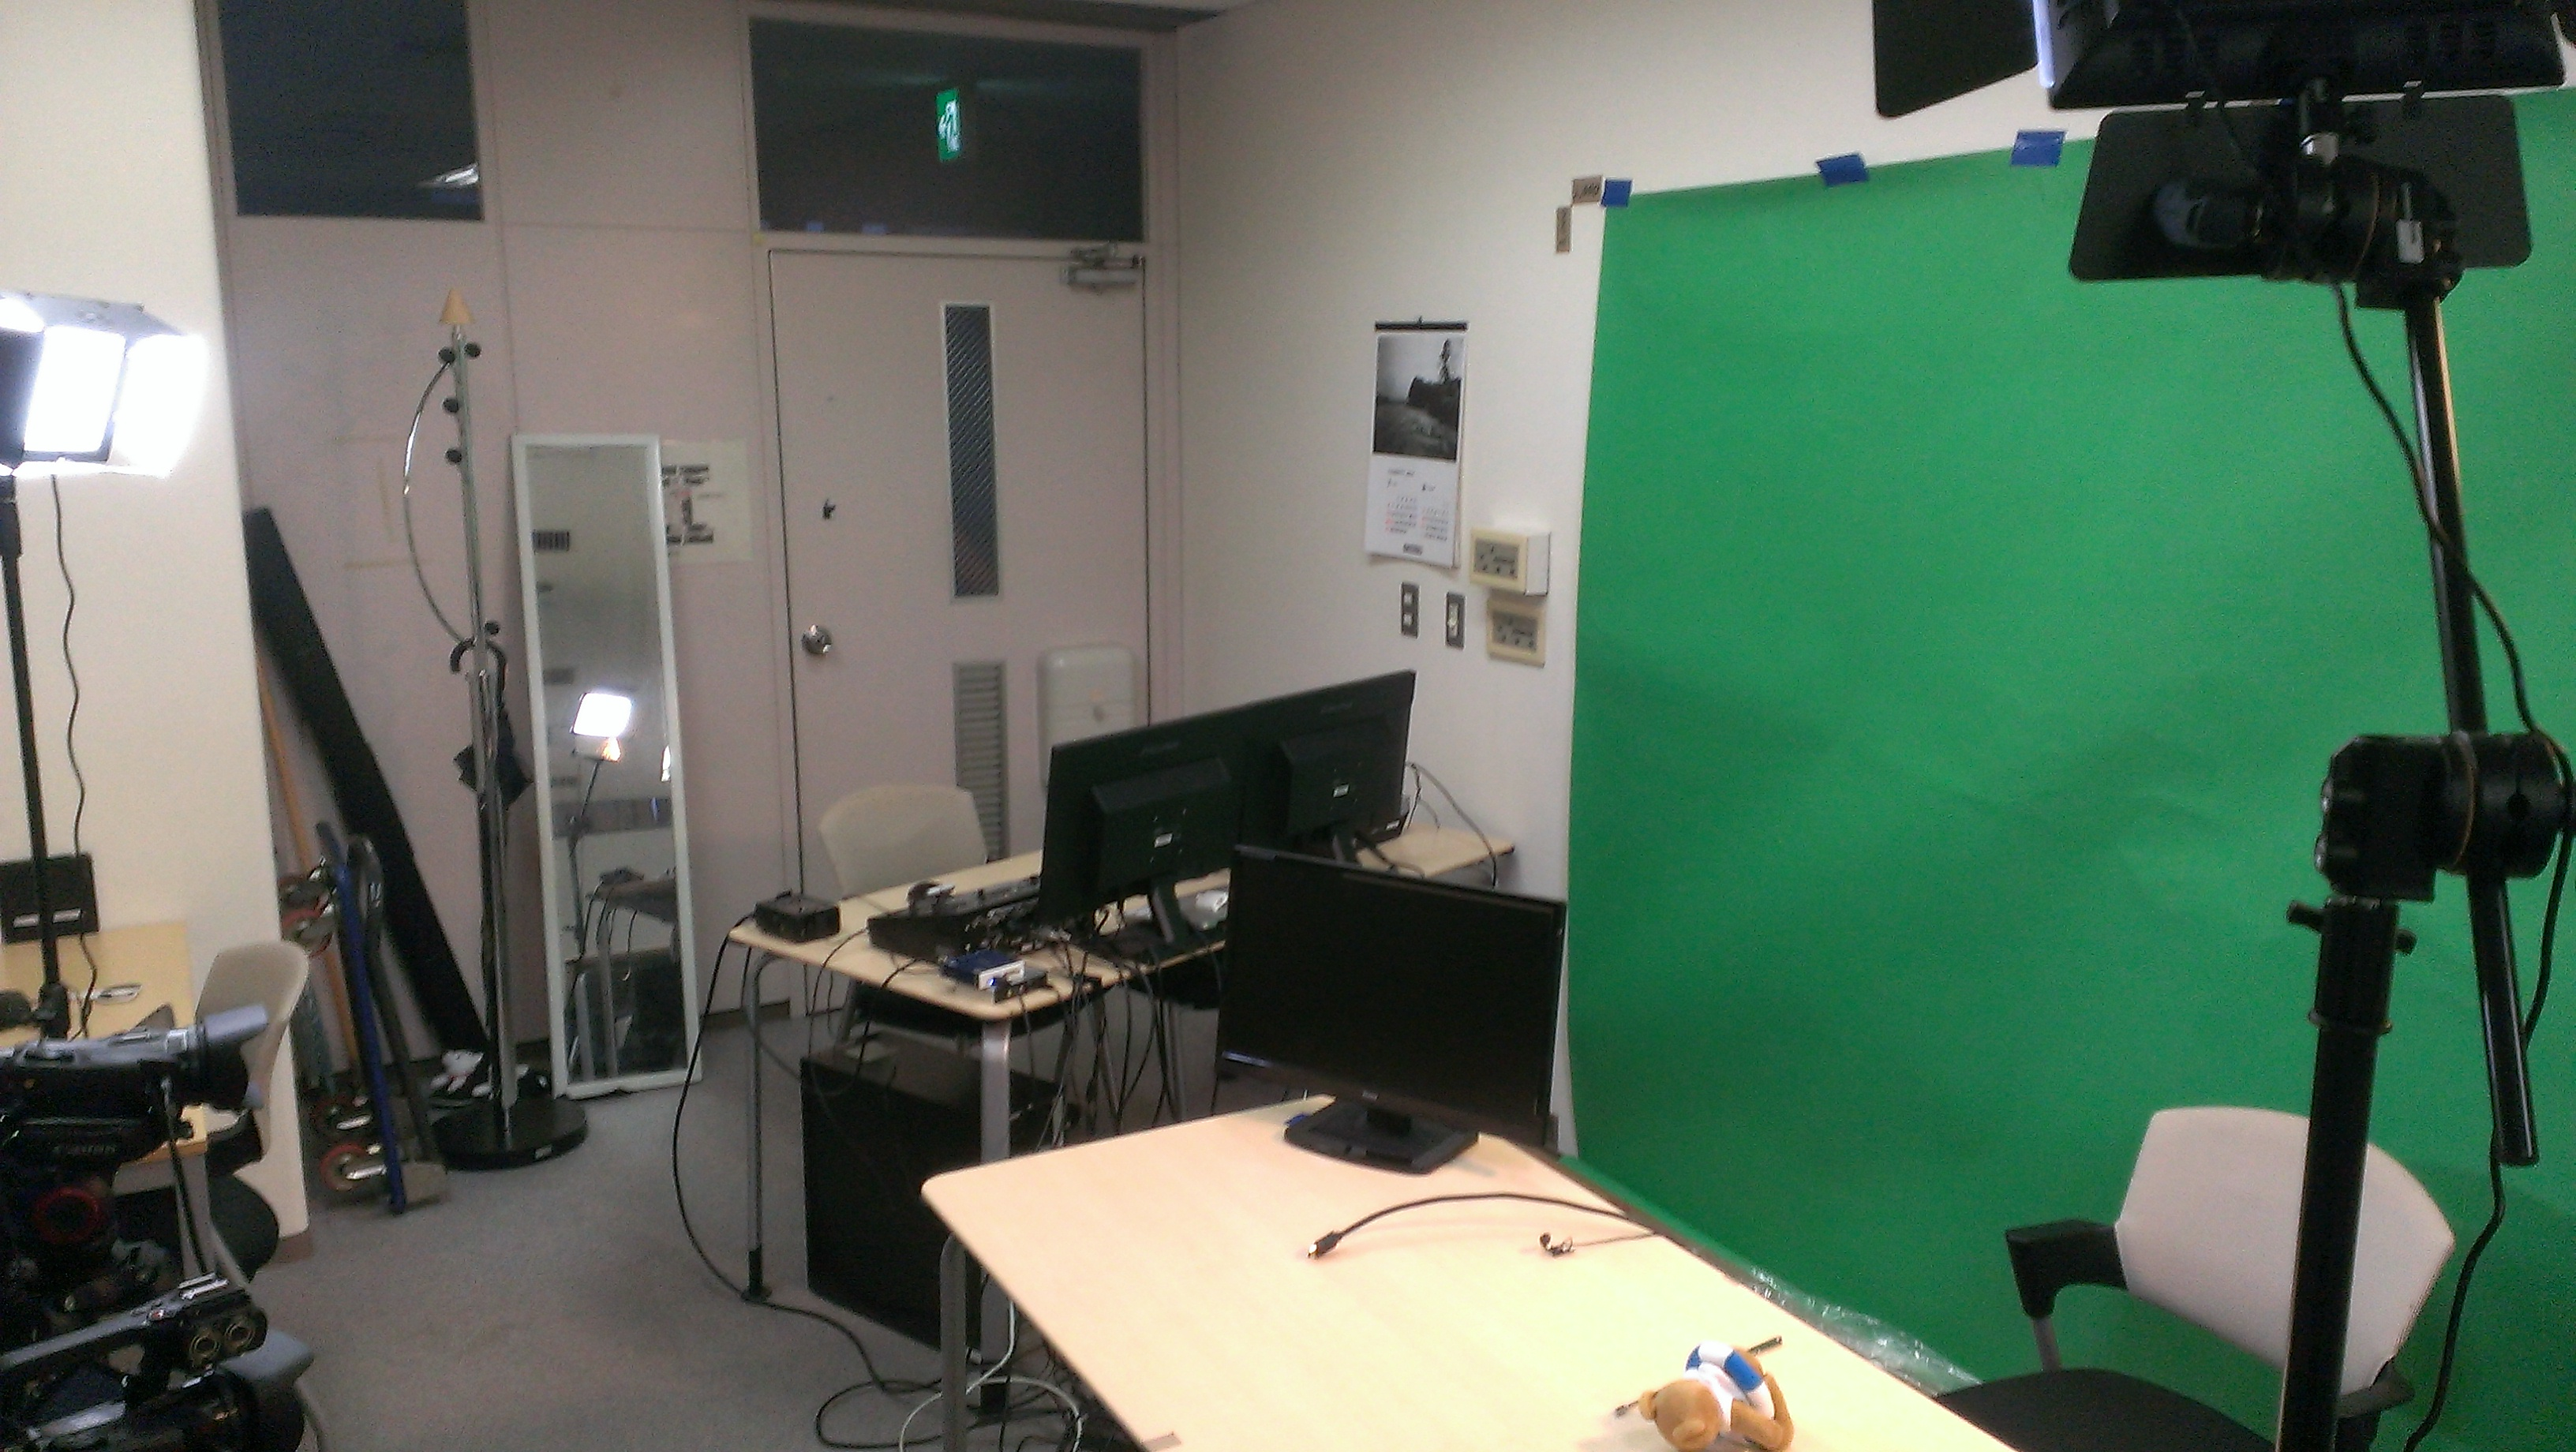
\includegraphics[width=\textwidth]{figures/lights.jpg}
 \caption{クロマキー合成のための背景紙および照明機材}
 \label{fig:lights}
\end{figure*}

また,このような教材を収録するために大掛かりな撮
影用スタジオを用意することは困難である.従って,
画像の背景としてセットを用意するようなことはでき
ない.このため,本研究ではクロマキー合成を利用し
て背景の画像を任意に合成できるようにした.この処
理は,前述のスイッチャーを利用して行うことができ
る.クロマキー合成を行うために,緑色の背景紙を用
いている.また,合成に際しては照明を適切に設置し
なくてはならない.この様子を図\ref{fig:lights}に
示す.



% \begin{figure*}
%  \centering
%  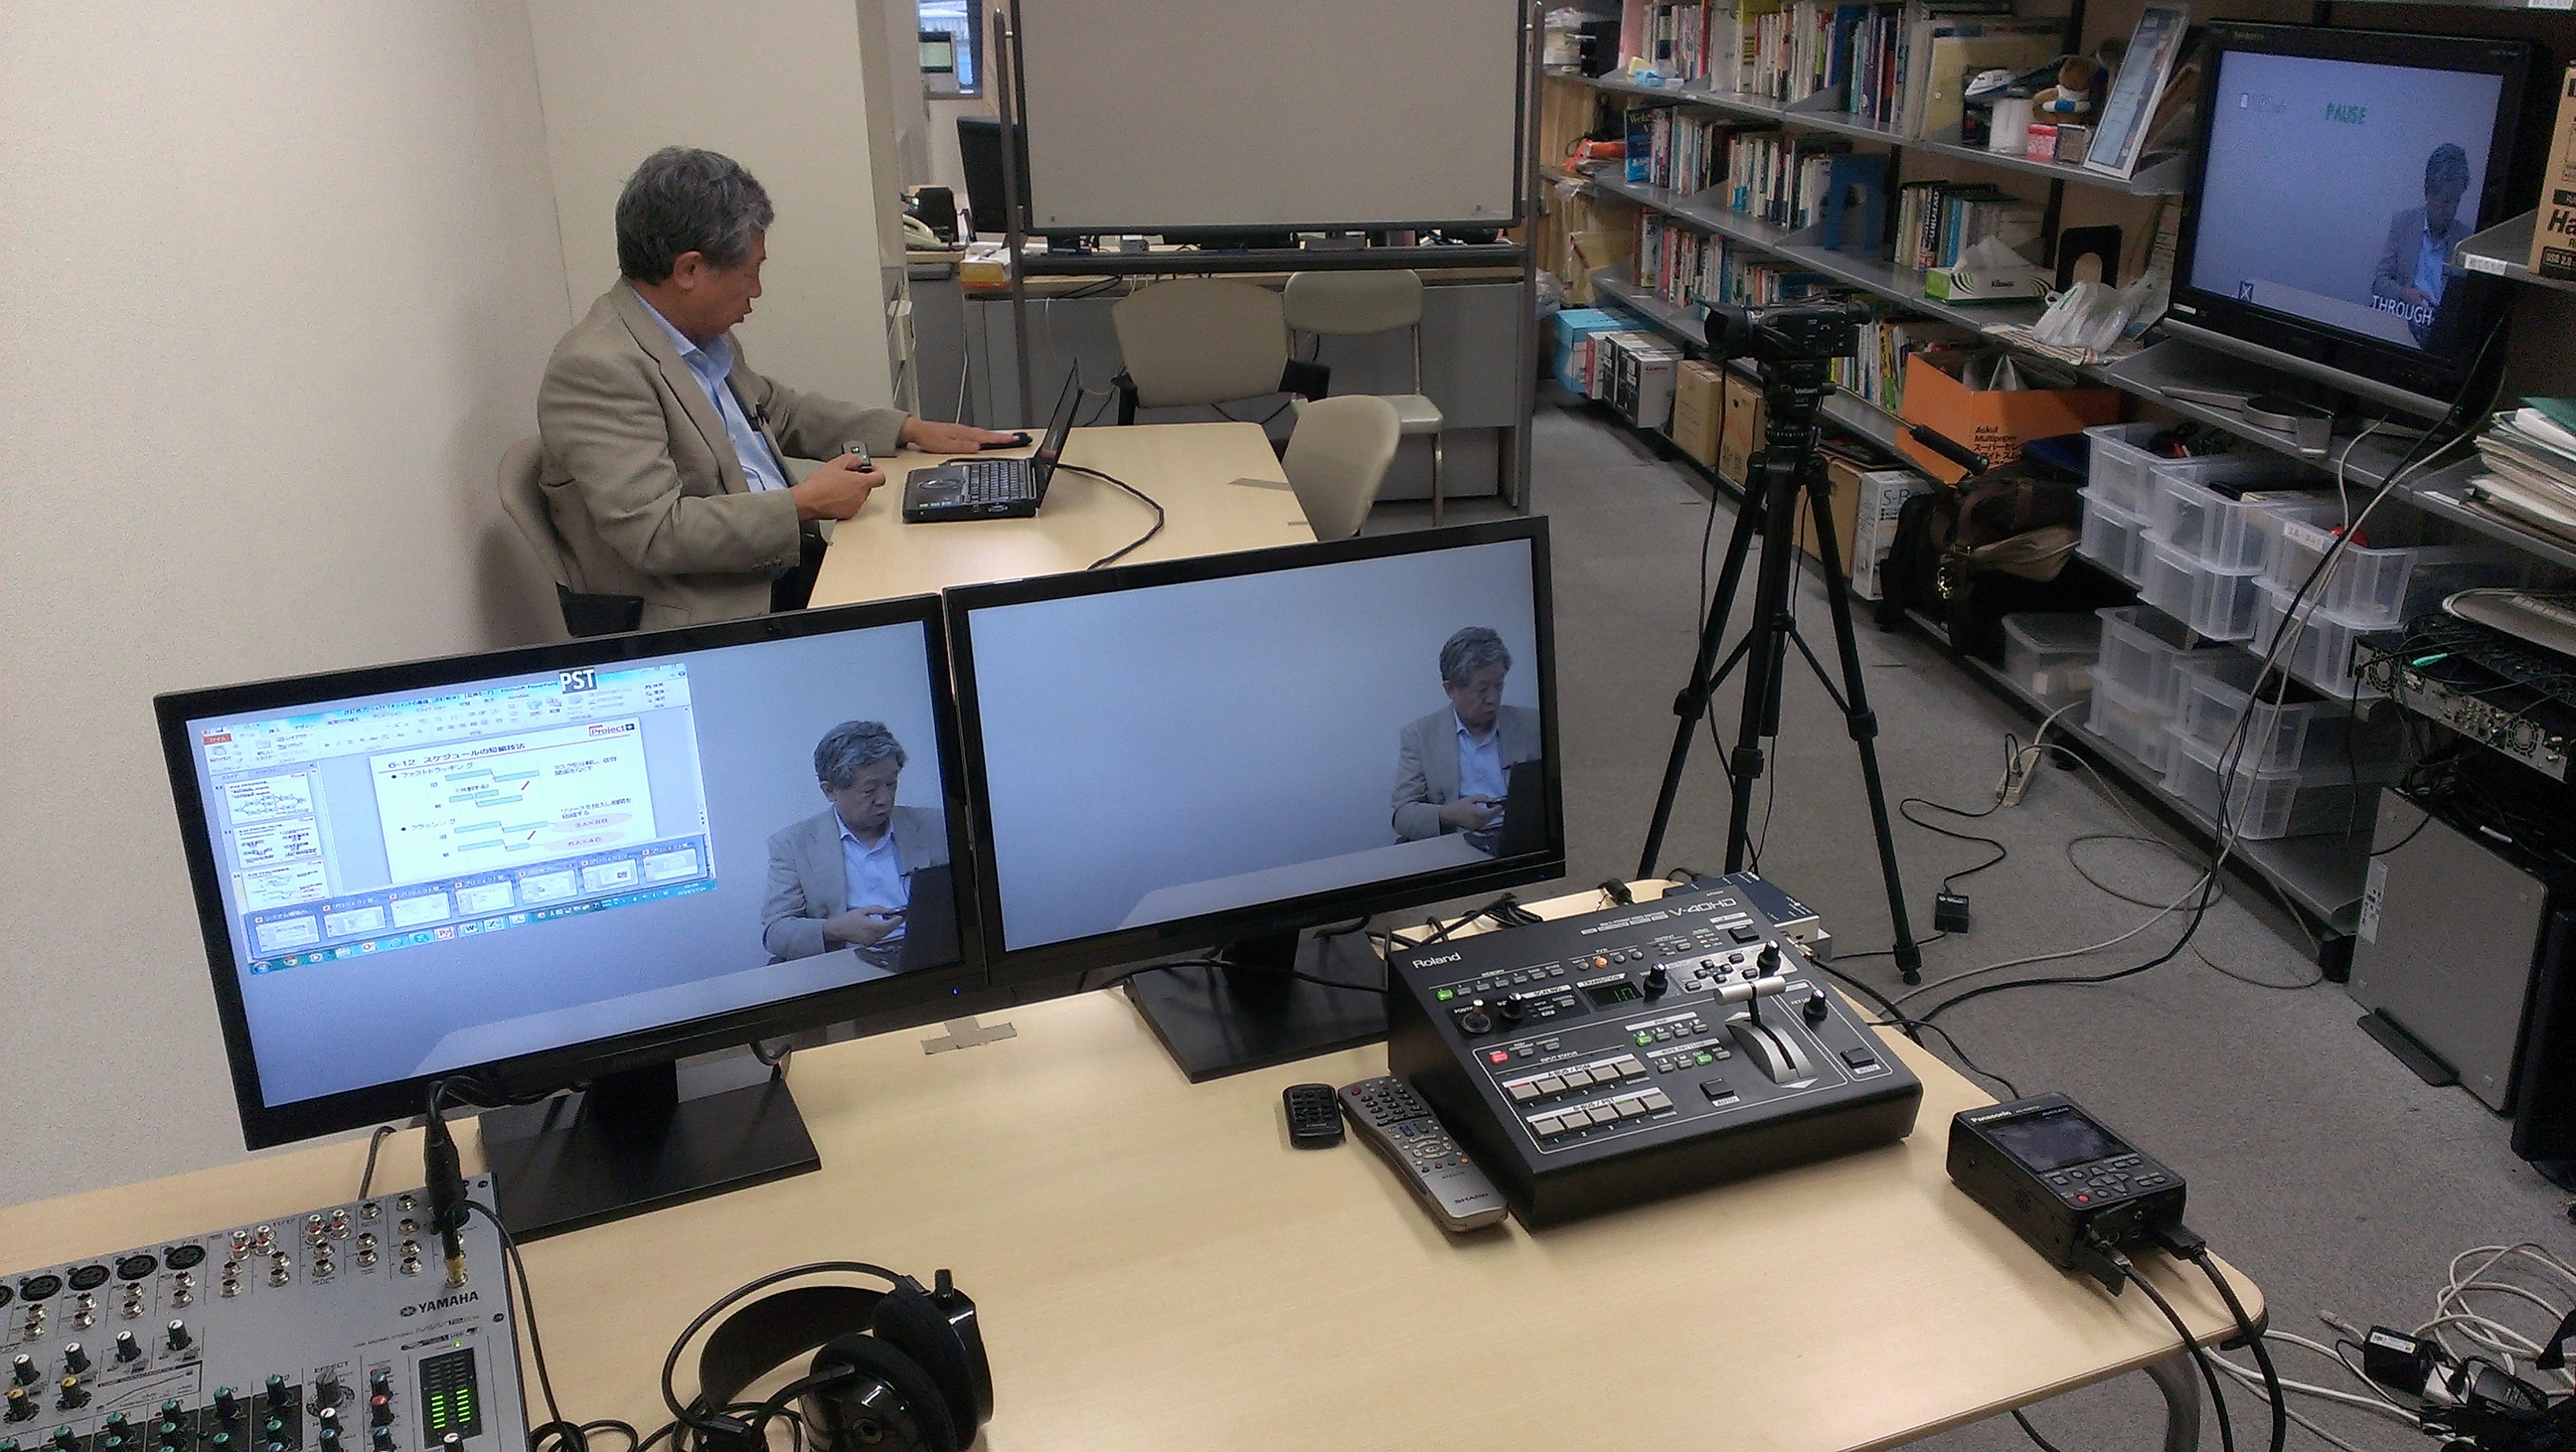
\includegraphics[width=\linewidth]{figures/recording.jpg}
%  \caption{アジャイル教材開発スタジオでの収録}
%  \label{fig:recording}
% \end{figure*}

\section{おわりに}
本稿では,本学enPiTプログラムにおける遠隔PBLの実
施とそのためのツールについて論じた.クラウド型開
発環境を利用することで,遠隔地のメンバーとの協働
によるソフトウエア開発を円滑に実施することができ
た.

このような技術を用いたPBLを実施するためには,利用
するツールについて事前に学習しておくとよい.これ
以外にも,PBLに必要となる様々な教材の開発が求めら
れる.特に,動画教材作成作業を容易にするためのア
ジャイル教材開発スタジオを構築した.

今後も,これらの知見を発展させ,より効果的なPBL型
学習を実施するための教材・教授法の研究開発を行
う.

\section{謝辞}
本研究の一部はJSPS科研費25330411の助成を受けたものである.

\bibliographystyle{junsrt}
\bibliography{bibliography/reference}
\end{document}

\clearpage
\section{はじめに}
本稿では産業技術大学院大学紀要の書式について記す.

\section{原稿}
\subsection{カメラレディ原稿}
原稿は,日本語もしくは英語による完全版下(camera ready)原稿とする.
製版後の校正は原則として不可能であるため,誤字や脱字がないよう,特に念
を入れて仕上げる.刷り上がりは,6頁以上が望ましい.

\subsection{余白}
天地左右余白(マージン)・段間余白(コラムスペース)はこの見本に従う.
上下の余白には製本時にヘッダとページ番号を挿入するので,空白にしておく
こと.

\section{標題について}
\subsection{標題}
標題は和文ならびに英文とする.英文原稿の場合は,和文表題を記述する箇所
に英文標題を記述し,英文標題の箇所は削除すること.

\subsection{アブストラクト・キーワード}
和文ではなく英文で記述すること.アブストラクトは80語程度とし,キーワー
ドは5つ程度とする.

\subsection{標題等の割付}
見本に従って,[和文標題,和文著者名,英文標題,英文著者名,英文アブスト
ラクト,英文キーワード]及び[受領日,所属]の割付を行う.

\subsection{英文原稿の場合}
英文による原稿の場合は,和文著者名のところに英文で記述し,英文著者名の
ところは削除すること.所属も英文で記述すること.

\section{本文について}

\subsection{句読点}
和文の句読点には全角ピリオド(.),全角コンマ(,)を用いること.

\subsection{見出し}
原稿には,大見出し,中見出しなどを設け,それらを明瞭に区分する.さらに
細分を要するときは著者に委ねる.

\section{参考文献について}
参考文献は,通し番号とし,本文中では,当該事項または人名などの参考とす
る後に,\cite{okumura},あるいは,\cite{takeuchi1986new,sutherland2011scrum} のよ
うに記す.文章の末尾に記す必要がある場合には,句読
点の前に記す\cite{IT人材白書2012}.

参考文献は,原則として,雑誌の場合は,著者,標題,雑誌名,巻,号,頁,
年の順に記す.また,書籍の場合は,著者,書名,発行所,発行年の順に記す.
参考文献例を本文の最後に挙げるので参考されたい.

\section{脚注等について}
\subsection{脚注}
脚注は段組の下部に記載する\footnote{脚注の例}.

\subsection{ルビ・圏点}
\ruby{難読漢字}{なんどくかんじ}にはルビを振ることができる.また,強調
したい箇所には\kenten{圏点をつける}ことができる.

\section{図・表について}
\subsection{図表のキャプション}
図・表には,図1,図2,表1,表2 のように論文全体で通し番号をつけること.
英文の場合には,Fig. 1,Fig. 2,Table 1,Table 2のように,番号をつける
こと.通し番号,標題は本文と同じ書体を使用すること.

表のキャプションは表の上に,図のキャプションは図の下につけること.

\begin{figure}
 \centering	% \begin{center} は使わない.余計な余白が入る.
 % 図を9行取り(9\baselineskip)して挿入する例
 
\includegraphics[height=9\baselineskip]{aiit_symbol.eps}
 \caption{図のキャプション}
 \label{fig:one}
\end{figure}

\subsection{図表に関する注意}
図・表は,印刷に十分耐えうるものでなければならない.刷り上がり時の文字
が小さすぎないよう十二分に配慮し,線の太さにも注意する.

図・表に色刷りを必要とする場合は,別途連絡すること.ただし,製本上の都
合で色刷り頁を設けることができない場合もありうる.

\begin{table}
 \centering
 \caption{表のキャプション}
 \begin{tabular}{c|ccc} \hline \hline
   & A & B & C \\ \hline
   R1 & $A_{1}$ & $B_{1}$ & $C_{1}$ \\
   R2 & $A_{2}$ & $B_{2}$ & $C_{2}$ \\
   R3 & $A_{3}$ & $B_{3}$ & $C_{3}$ \\
   R4 & $A_{4}$ & $B_{4}$ & $C_{4}$ \\ \hline
 \end{tabular}
 \vskip 10pt % 左右の段の行が揃うように調整
\end{table}

\section{テンプレート}
\LaTeX を利用する執筆者は,\texttt{aiit\_bulletin.tex}を書き換えて使う
こと.また,MS Wordを利用する場合は,\texttt{aiit\_bulletin.docx}ファイ
ルを用いること.

\section{おわりに}
本稿では産業技術大学院大学紀要のフォーマットについて記した.

\appendix
\section{注意事項}
\subsection{フォントの準備}
LaTeXとWordで同じ字体に揃えるため,和文には「IPAexフォント(2書体パッ
ク)」を用いる.次のサイトからインストールすることができる.

\url{http://ipafont.ipa.go.jp/ipaexfont/download.html}

なお,TeX Live 2012 以降およびW32TeX [2013/06/06] 以降の
luatexja.tar.xzに は同梱されている.

\subsection{版面と余白}
何らかの事情で書式を自分で設定する場合,本文の書式は次の通りとする.

\begin{itemize}
 \item フォントの大きさは8.5pt(=12Q) とする.
 \item 2段組とし1行27文字で,段間は2文字分あける.
 \item 行間は字の高さの75\%とし,1頁47行とする.
 \item 余白は天(上部)30mm,ノド(内側)25mmとする.
\end{itemize}

これら以外の書式は可能な限りこの見本に合わせる.

